\documentclass{article}
\usepackage[a4paper]{geometry}
\usepackage{hyperref}
\usepackage{pgfplotstable}
\usepackage{pgfplots}
\usepackage{courier}
\usepackage{amsmath,amsfonts,amssymb,mathtools}

\newcommand{\code}[1]{\texttt{#1}}
\newcommand{\figref}[1]{\href{fig:#1}{Figure #1}}
\newcounter{example}
\newcommand{\example}{\stepcounter{example}\paragraph{Example \theexample}}

\hypersetup{
    colorlinks=true
}

\title{\textbf{Lecture 2: An Optimization View to Fit the Best Line}}
\author{Bhaya, A.G.\thanks{Electronic Mail: \href{mailto:contact@angubh.io}{\code{ananya.gb@nbu.ac.in}}}
}

\pgfplotsset{compat=1.18}
\begin{document}
    \maketitle
    \tableofcontents

    \section{Introduction}
    Consider the three data points shown in \figref{1}. For the given set, it may not be possible to fit a line that passes through all the three points. So, it would be impossible a ML algorithm to design a function that creates a line passing through all the points. In such a case, one should create a line that minimizes the error, when defining relationships between coordinates. Such a line is called a \textbf{best-fit line}.

    \begin{figure}[ht]
        \centering
        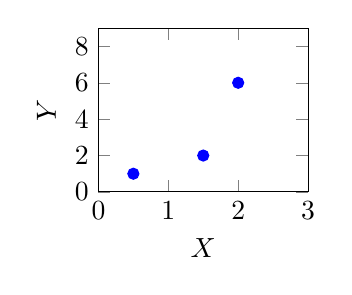
\begin{tikzpicture}
        \begin{axis}[
            xlabel={$X$},
            ylabel={$Y$},
            grid=minor,
            xmin=0, xmax=3,
            ymin=0, ymax=9,
            width=0.35\textwidth
        ]
        
        % Add the plot of the function
        \addplot[
            only marks,
            color=blue,
            mark=*,
            ]
            coordinates {
            (0.5,1)(1.5,2)(2,6)
            };
        
        \end{axis}
    \end{tikzpicture}
        \caption{A scatter graph of three data points.}
        \label{fig:1}
    \end{figure}

    \section{Best-Fit Line}

    For the given points in \figref{1}, one could plot the best possible line as shown in \figref{2}. In the given figure, the line drawn in red is the best-fit line.

    But on what grounds is it a best fit line? The best fit line is drawn in such a way, that the squares of the distances between the line and the given points is minimized, or in other words the error is minimized.

    Considering the best fit line is \(\hat{y}=ax+b\), the error, \(E\) is,

    \begin{equation}
        E=\sum_{i=1}^n{(y_i-\hat{y}_i)^2}=\sum_{i=1}^n{(y_i-ax_i-b)^2}
    \end{equation}

    \begin{figure}[ht]
        \centering
        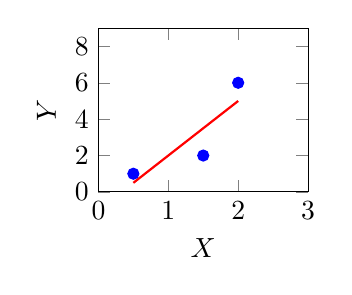
\begin{tikzpicture}
        \begin{axis}[
            xlabel={$X$},
            ylabel={$Y$},
            grid=minor,
            xmin=0, xmax=3,
            ymin=0, ymax=9,
            width=0.35\textwidth
        ]
        
        % Add the plot of the function
        \addplot[
            only marks,
            color=blue,
            mark=*,
            ]
            coordinates {
            (0.5,1)(1.5,2)(2,6)
            };
        \addplot[
        red,
        thick,
    ]
    table[
        y={create col/linear regression={
            x=x,
            y=y
        }}
    ] {
        x y
        0.5 1
        1.5 2
        2   6
    };
        
        \end{axis}
    \end{tikzpicture}
        \caption{A potential best-fit line shown in red.}
        \label{fig:2}
    \end{figure}
    
    \begin{example}
        Find the best straight line fit to the three points \((x,y)=\{(-1,-2),(0,0),(1,3)\}\).
    \end{example}

    \subparagraph{Solution}
    Let \(y=ax+b\) be the straight line. We can write the data matrix for the given points as, \(A=\begin{bmatrix}
            -1 & 1\\
            0 & 1\\
            1 & 1
        \end{bmatrix}\), and the solution matrix, \(b=\begin{bmatrix}
            -2\\
            0\\
            3
        \end{bmatrix}\). Considering, \(x=\begin{bmatrix}
            a\\
            b
        \end{bmatrix}\).

        The loss function is given by, \(L(x)=(Ax-b)^T(Ax-b)\). Upon differentiating the loss function, we get, \(\nabla L(w)=2A^T(Ax-b)=0\). Hence, \(A^TAx=A^Tb\).

        \begin{align*}
            A^TA&=\begin{bmatrix}
                -1 & 0 & 1\\
                1 & 1 & 1
            \end{bmatrix}\begin{bmatrix}
                -1 & 1\\
                0 & 1\\
                1 & 1
            \end{bmatrix}=\begin{bmatrix}
                2 & 0\\
                0 & 3
            \end{bmatrix}\\
            \textnormal{and, }
            A^Tb&=\begin{bmatrix}
                -1 & 0 & 1\\
                1 & 1 & 1
            \end{bmatrix}\begin{bmatrix}
                -2\\
                0\\
                3
            \end{bmatrix}=\begin{bmatrix}
                5\\
                1
            \end{bmatrix}
        \end{align*}

        Upon creating augmented matrix for \(A^TAx=A^Tb\), we get,

        \begin{align*}
            \left[
                \begin{array}{cc|c}
                    2 & 0 & 5\\
                    0 & 3 & 1
                \end{array}
            \right]\xrightarrow{\textnormal{Row reduction}}
            \left[
                \begin{array}{cc|c}
                    1 & 0 & \frac{5}{2}\\
                    0 & 1 & \frac13
                \end{array}
            \right]
        \end{align*}

        Therefore, \(x=\begin{bmatrix}
            a\\
            b
        \end{bmatrix}=\begin{bmatrix}
            \frac52\\
            \frac13
        \end{bmatrix}\). The best fit line is given by, \(y=\dfrac52x+\dfrac13\).

        \pagebreak

        \begin{example}
            Find the best straight line fit to the three points \((x,y)=\{(-1,-2),(0,0),(1,3)\}\) using calculus optimization.
        \end{example}

        \subparagraph{Sol.}

        The loss function (which gives mean squared error), is given by,
        
        \[L(w)=\displaystyle{\sum_{i=1}^{n}(y_i-\hat y_i)^2=\sum_{i=1}^{n}\{y_i-(ax_i+b)\}^2}\]

        The best fit line is the one which has the lowest possible value of \(L(w)\). Since, there are two parameters, we minimize \(L(w)\) using \(a\), and \(b\) using partial differentiation.

        \begin{align*}
            \frac{\partial L(w)}{\partial a}&=\frac{\partial}{\partial a}\sum_{i=1}^n{\{y_i-(ax_i+b)\}^2}=0\\
            &\Rightarrow \sum_{i=1}^nx_i\{y_i-(ax_i+b)\}=0\\
            &\Rightarrow -1(-2+a-b)+0+(3-a-b)=0\\
            &\Rightarrow 2a=5\Rightarrow a=\frac{5}{2}
        \end{align*}

        Similarly, for \(\nabla_b L(w)=0\), \(b=\dfrac13\). Hence the best fit line is, \(y=\dfrac52x+\dfrac13\).

        \paragraph{Linear Algebra Overview}

        In terms of linear algebra, the loss function \(L(w)\) can be written as, \(L(w)=||Ax-b||^2\), where \(Ax-b\) is a scalar quantity. In terms of matrices, \(L(w)=(Ax-b)^T(Ax-b)\). To find the best fit line, we minimize \(L(w)\), which gives us \(\nabla L(w)=2(Ax-b)^TA=2A^T(Ax-b)=0\) Hence we can equate, \(A^TAx=A^Tb\), to find the parameters.
\end{document}.